\documentclass[a4paper]{article}
\usepackage[utf8]{inputenc}
\usepackage{underscore}
\usepackage[english,serbian]{babel}
\usepackage{graphicx}
\usepackage{color}
\usepackage{url}
\usepackage{float}
\usepackage[unicode]{hyperref}
\usepackage[table]{xcolor}
\hypersetup{colorlinks, citecolor=green, filecolor=green, linkcolor=blue, urlcolor=blue}

\begin{document}



\title{Pametni (elektricni) automobili u 2022. godini\vspace{3ex}\\
\small{Seminarski rad u okviru kursa\\
Tehničko i naučno pisanje\\
Matematički fakultet}\vspace{3ex}}
\author{\\\\\\Nera Zejak\\Eleonora Jovanovic Kisseleva\\Nemanja Potic\\Kristijan Petronijevic \\ \\nerazejak1130@gmail.com\\eleonorajovanovic1@gmail.com\\x.nemanjapotic.x@gmail.com\\ petronijevick3@gmail.com\\}
\date{13.~novembar 2022.}\
\maketitle

\maketitle



\abstract{
    U narednom tekstu cemo se ukratko upoznati sa \textbf{Pametnim (elektricnim) automobilima.} Pocev od toga sta su pametni automobili, objasnićemo šta su osnove bioinformatike, kao i mnoge zanimljive činjenice ove jedinstvene interdisciplinarne oblasti. Razgovaramo o glavnim principima koji podupiru bioinformatičke analize, razmatramo tipove bioloških informacija i baza podataka koje se obično koriste.}

\newpage

\tableofcontents
\newpage

\section{Uvod}
   Električni automobil je automobil koji se pokreće elektromotorom, koristeći \textbf{električnu energiju} pohranjenu u akumulatoru, ili drugim uređajima za pohranu energije. Električni automobili su bili popularni krajem 19. i početkom 20. veka. 
        


\begin{figure}[h]
        \centering
        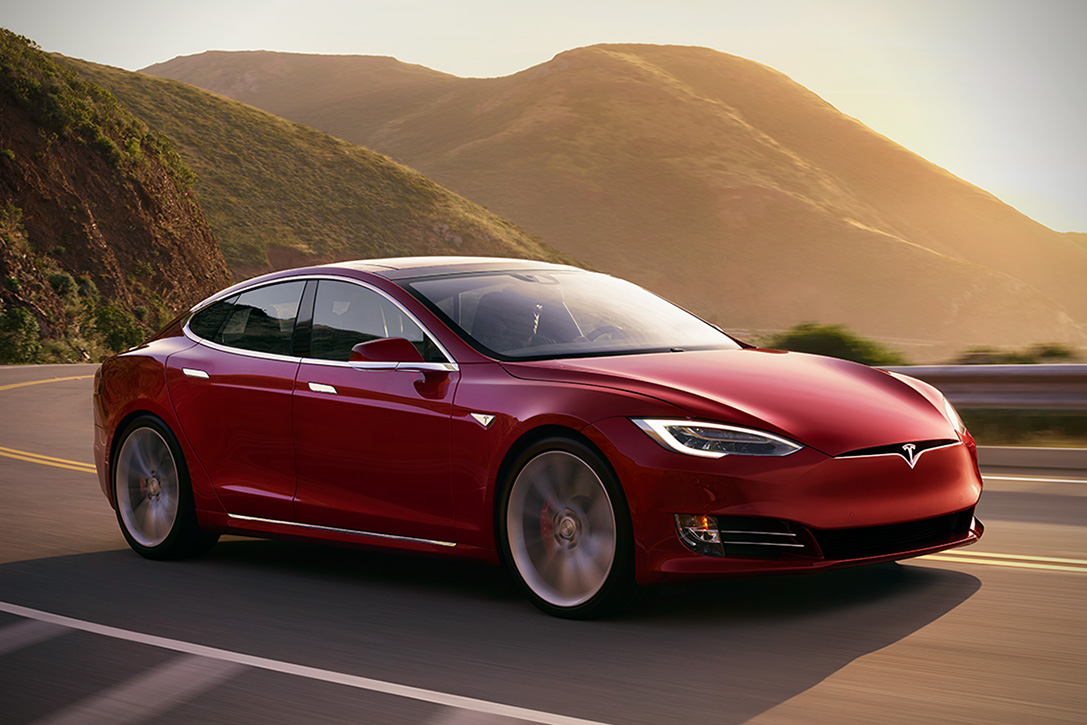
\includegraphics[width=\linewidth]{tesla.jpeg}
        \caption{Tesla model S}
        \label{fig:my_label}
        \end{figure}
        Unapređenja motora sa unutarnjim sagorevanjem i masovna proizvodnja jeftinijeg vozila na benzin doveli do smanjenja korištenja vozila na električni pogon.
         Energetske krize 1970-ih i 80-ih dovele su do kratkotrajnog zanimanja za \textbf{električne automobile}, te se sredinom 2000. obnovio interes za proizvodnjom električnih automobila, uglavnom zbog zabrinutosti oko ubrzanog povećanja cene nafte i potrebe za smanjenjem emisije gasova staklene bašte.
         
\label{sec:uvod}

\newpage
\section{Drugi naslov}

\rowcolors{2}{gray!10}{gray!40}
\resizebox{\textwidth}{!}{
\begin{tabular}{|l|c|r|}
    \hline
     \cellcolor{purple}
    A & B & \cellcolor{purple} C \\
    \hline
    D & E & F \\
    \hline
    G & H & I \\
    \hline
\end{tabular}}

slika tesle https://hiconsumption.com/tesla-model-s-p100d/
\end{document}

